% Section content template for individual Educative lessons
% This file contains the actual content for a specific section
% Generated from Educative API section content

% Section: Use Case Diagram for the Amazon Locker Service
% Section ID: 6219731115966464
% Section Slug: use-case-diagram-for-the-amazon-locker-service
% Generated: 2025-12-11T15:16:35.434691

Let's build the use case diagram of the Amazon Locker System and understand the relationship between its main actors and functions. First , we'll define the different elements of our system, followed by the complete use case diagram.

\subsection{System}\label{8w1-aQk_z4wkRYZ9OQ3k-}
\\
Our system is the Amazon Locker system. It manages automated package deliveries and returns via secure locker locations.

\subsection{Actors}\label{qGKhgJJDLAV05SZrzh_mL}
\\
Now, we'll define the main actors of our Amazon Locker system.

\subsubsection{Primary actors}\label{_jJtzQF2Dz_Fy8jHIqCrv}

\begin{itemize}
\item
\protect\phantomsection\label{yACOIiavU5o9TkSBY-Sd-}
\textbf{Customer:} This Amazon customer ordered a package delivered to the Amazon Locker. The customer is responsible for selecting and booking a locker location for their order delivery. This actor can enter the code at the locker to retrieve their product, request a return, and drop off the package.
\item
\protect\phantomsection\label{6LA16ZRA-pXpAElfXl7cK}
\textbf{Delivery person:} This actor can also enter the code and add the product to the locker so the ``Customer'' can pick it up. This actor can also pick up a returned package from the locker. The delivery person uses unique, one-time codes for each delivery or return.
\end{itemize}

\subsection{Use cases}\label{UUHa-1klk8FSwQJ7u5PuP}
\\
This section defines locker use cases. We have listed them according to their respective interactions with a particular actor.
\begin{quote}
\textbf{Note:} Some use cases will occur multiple times because they are shared among different actors in the system.
\end{quote}
\subsubsection{Customer}\label{I8o3iKF7m3wpKlbGSCcys}

\begin{itemize}
\item
\protect\phantomsection\label{eCsS9jUuagLJnhh9_1Ngg}
\textbf{Select locker location:} Tochoose a preferred location for package delivery or product return.
\item
\textbf{Pick up package:} Toretrieve the delivered package from the locker after unlocking it.
\item
\textbf{Remove package:} To collect a package from the locker after delivery or for return.
\item
\textbf{Add package:} To use the provided access code to place a return package inside the locker.
\item
\textbf{Submit return request:} To start the process to return a purchased product through a locker.
\item
\textbf{Receive delivery notification:} To get notified when a package has been delivered to the assigned locker, including locker details and access code.
\item
\textbf{Receive return notification:} To get notified with instructions and code for returning a product via a locker.
\item
\protect\phantomsection\label{eCsS9jUuagLJnhh9_1Ngg}
\textbf{Receive overdue notification:} To get notified if the package was not picked up before the deadline.
\end{itemize}

\subsubsection{Delivery person}\label{nexBjcJkJ7gShhOIgvIVa}

\begin{itemize}
\item
\textbf{Deliver package:} To place a customer's package inside the assigned locker for pickup.
\item
\textbf{Remove package:} To retrieve returned items from the locker for processing or transport.
\item
\protect\phantomsection\label{cw3s-91-jiBSlpGeXs-UQ}
\textbf{Receive return notification:} To get alerted about packages that have been returned and are ready for pickup.
\end{itemize}

\subsubsection{System}\label{Rm9pWE5U_qFi4rWgMbNj5}

\begin{itemize}
\item
\textbf{Issue locker:} To assign a suitable locker to a package based on size and availability.
\item
\textbf{Generate code:} To create a unique access code for locker entry.
\item
\textbf{Validate code:} To check if the entered code is correct and valid for locker access.
\item
\textbf{Find locker:} To locate the correct locker corresponding to the access code.
\item
\textbf{Lock/unlock locker door:} To control the mechanism to secure or open the locker door.
\item
\textbf{Send delivery notification:} To inform the customer that their package has been delivered and provide locker details and code.
\item
\textbf{Send return notification:} To notify the delivery person about returned products that require pickup.
\item
\protect\phantomsection\label{VeaWCJjXOTZR19XJcx-jB}
\textbf{Send overdue notification:} To alert the customer when a package hasn't been collected within the specified time frame.
\end{itemize}

\subsection{Relationships}\label{15sE70CpzILojoobSA_Zu}
\\
This section describes the relationships between and among actors and their use cases.

\subsubsection{Associations}\label{v05pu51kpwwl89icVbRMd}
\\
The table below shows the association relationship between actors and their use cases.

\begin{center}
\begin{tabular}{|p{0.3\linewidth}|p{0.3\linewidth}|p{0.3\linewidth}|}
\hline
\textbf{Customer} & \textbf{Delivery Person} & \textbf{Amazon Locker System} \\
\hline
Select locker location & Deliver package & Issue locker \\
\hline
Pick up package & Remove package & Generate code \\
\hline
Submit return request & Add package & Remove package \\
\hline
Find locker & Lock/unlock locker door & Validate code \\
\hline
Receive delivery notification &  & Receive return notification \\
\hline
 &  & Send delivery notification \\
\hline
 &  & Send return notification \\
\hline
 &  & Receive overdue notification \\
\hline
 &  & Send overdue notification \\
\hline
\end{tabular}
\end{center}



\subsubsection{Include}\label{E6c3ykAkGs3AZ07d6dOGz-2}
\\
When a customer picks up, adds, or removes a product from a locker, or when a delivery person delivers a package, they must first enter a code. The system checks the code's validity, locates the appropriate locker, and unlocks the door. These are best represented using ``include'' relationships in a use case diagram:

\begin{itemize}
\item
\protect\phantomsection\label{OfUNUCxwWKittyr7SiTJF}
``Pick up package,'' ``Add package,'' ``Deliver package,'' and ``Remove package'' use cases all include the ``Enter code'' use case.
\item
\protect\phantomsection\label{jL326-F4R4eAHopjBwZPi}
``Enter code'' includes ``Validate code'' use case.
\item
\protect\phantomsection\label{HvqscalyXvPC6BG-j20qA}
``Validate code'' includes ``Find locker.''
\item
\protect\phantomsection\label{MCvf6s1JhCDPlnCg1O5jK}
``Find locker'' includes ``Lock/unlock locker door.''
\end{itemize}
\\
For product returns, the customer initiates the process on the Amazon Locker system by submitting a return request. After the request is approved, the Amazon Locker system sends a return notification and generates a unique code for locker access.

\begin{itemize}
\item
\protect\phantomsection\label{CP4oJX1gW5Tn4KpkQvajV}
The \textbf{``} Submit return request''use case includes the``Send return notification''use case.
\item
\protect\phantomsection\label{Sz8rr_eYtL5tY4wdphito}
The \textbf{``} Send return notification''use case includes the``Generate code''use case.
\end{itemize}
\\
The system generates the required access code when a locker is assigned for an order.

\begin{itemize}
\item
\protect\phantomsection\label{sSh_tRzZFXC8El003g0uf}
The ``Issue locker'' use case includes the ``Generate code'' use case.
\end{itemize}

\subsection{Use case diagram}\label{SxGi5p0Ff11tQgi3hhBbm}
\\
Here's the use case diagram for the Amazon Locker system:

\begin{figure}[htbp]
 \centering
 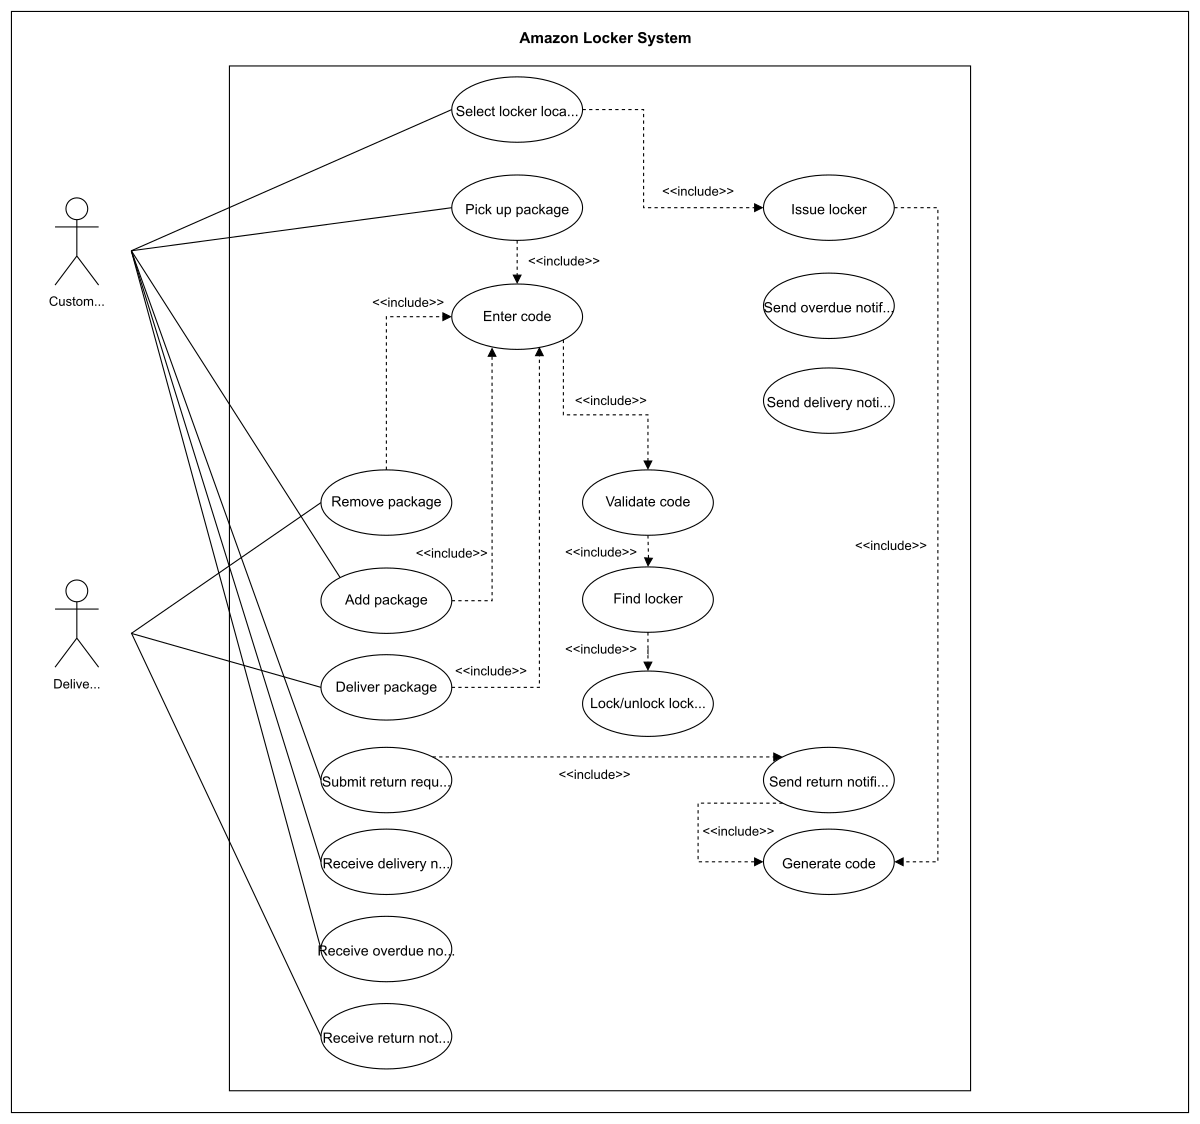
\includegraphics[width=0.5\textwidth]{Images/chapter_10/section_6219731115966464/4968248104583168.png}
 \caption{The use case diagram for the Amazon Locker system}
\end{figure}

In the next lesson, we will discuss the class diagram with a detailed explanation of all classes and their relationship with each other.

% End of section content